\documentclass[11pt,a4paper]{article}

\usepackage[margin=1in]{geometry}
\usepackage{amsmath,amssymb,amsthm}
\usepackage{graphicx}
\usepackage{booktabs}
\usepackage{caption}
\usepackage[hidelinks]{hyperref}
\usepackage[T1]{fontenc}
\usepackage[protrusion=true,expansion=false]{microtype}
\usepackage{natbib}
\bibliographystyle{plainnat}

\newtheorem{theorem}{Theorem}[section]
\newtheorem{proposition}[theorem]{Proposition}
\theoremstyle{remark}
\newtheorem{remark}[theorem]{Remark}

\newcommand{\Q}{\mathbb{Q}}
\newcommand{\PP}{\mathbb{P}}
\newcommand{\E}{\mathbb{E}}
\newcommand{\Filt}{\mathcal{F}}
\newcommand{\dd}{\,\mathrm{d}}
\newcommand{\IV}{\mathrm{IV}}
\newcommand{\RV}{\mathrm{RV}}
\newcommand{\VRP}{\mathrm{VRP}}

\captionsetup{font=small,labelfont=bf}

\title{\bfseries Recovering the Pricing Kernel from Index Options:\\[0.3em]
\large An Estimation Exercise on the Radon--Nikodym Derivative}
\author{Aryan Bhujbal\thanks{Code and data-processing scripts:
\url{https://github.com/aryanbhujbal24/pricing-kernel}. All results in this
paper are reproduced by running the five numbered scripts in order.}}
\date{September 2026}

\begin{document}
\maketitle

\begin{abstract}
\noindent
Option prices identify the risk-neutral density $q$ of a future index level;
historical returns identify the physical density $p$. Their ratio is, up to
discounting, the projection of the Radon--Nikodym derivative $\dd\Q/\dd\PP$
onto the terminal index level. This paper estimates that object from SPX
options and quantifies how much of it the data actually determines.

Four results. First, the Breeden--Litzenberger estimator is consistent at
order $h^2$ but ill-posed: we derive the noise amplification analytically and
confirm on live quotes that naive second differencing of SPX mids yields a
density with a noise-to-signal ratio of $47$ and $39\%$ negative mass. Second,
an arbitrage-constrained SVI fit removes this entirely, producing a density
integrating to $0.99997$ whose mean matches the forward to $7\times10^{-5}$.
Third, the estimated pricing kernel is non-monotone at the point estimate --
the pricing-kernel puzzle -- but its shape reverses within the $95\%$ confidence
interval of the equity premium, so \emph{the puzzle is not identified at this
sample size}. Fourth, we reconstruct the VIX from our own chain to within
$0.07\%$, and show that the jump correction to the log-contract replication is
$12.3\%$ of implied variance, roughly $47\%$ of the measured variance risk
premium. Newey--West inference reduces the premium's $t$-statistic from $21.3$
to $5.5$.

\medskip
\noindent\textbf{Keywords:} pricing kernel, risk-neutral density,
Breeden--Litzenberger, SVI, variance risk premium, Radon--Nikodym derivative.
\end{abstract}

\section{Introduction}

Most empirical option work prices a contract under $\Q$. This paper does
something different: it treats the change of measure itself as the object of
estimation. The quantity of interest is
\begin{equation}
M(x) = e^{-rT}\,\frac{q(x)}{p(x)},
\end{equation}
the pricing kernel projected onto the terminal index level, where $q$ is
extracted from a cross-section of option prices and $p$ from a time series of
returns. Theory predicts $M$ should decrease in wealth. A substantial empirical
literature -- \citet{jackwerth2000}, \citet{aitsahalia2000},
\citet{rosenberg2002} -- finds it does not, a finding known as the pricing
kernel puzzle.

Our contribution is less a new estimate than a careful accounting of what the
data supports. Three methodological points organise the paper.

\paragraph{The extraction is an ill-posed inverse problem, and we measure how
badly.} Section~\ref{sec:theory} derives the noise amplification of the
Breeden--Litzenberger second difference in closed form; Section~\ref{sec:synth}
validates it against known densities; Section~\ref{sec:surface} confirms the
prediction on live SPX quotes. The naive estimator is not merely noisy -- on a
five-point strike grid the noise exceeds the signal by a factor of $47$.

\paragraph{The physical density must be conditional.} A kernel density on
historical horizon returns is \emph{unconditional}: it describes an average day
since 1990, when volatility averaged $18\%$. Our $q$ is conditional on a day
when implied volatility was $13.5\%$. Dividing one by the other measures the
gap between today and an average day. We report both estimators and treat their
difference as a result.

\paragraph{The headline finding is a negative one.} The estimated kernel is
non-monotone. But the physical drift enters directly, and the equity premium is
estimated with a standard error of $2.97\%$ per year. Sweeping the drift across
its own confidence interval flips the kernel from strongly non-monotone to
essentially monotone decreasing. We therefore cannot reject monotonicity, and
we argue that a point estimate reported without this sensitivity claims a
discovery the data has no power to make.

Section~\ref{sec:theory} derives the required results. Section~\ref{sec:synth}
validates the estimator on synthetic data. Section~\ref{sec:data} describes the
data. Sections~\ref{sec:surface}--\ref{sec:vrp} present the surface, the
kernel, and the variance risk premium. Section~\ref{sec:limits} states the
limitations; Section~\ref{sec:conclusion} concludes.

\section{Theory}
\label{sec:theory}

\subsection{Setup and the projected kernel}

Fix a horizon $T$ and a filtered probability space
$(\Omega,\Filt,(\Filt_t),\PP)$. Let $S_t$ be an index paying continuous
dividend yield $q_d$, let $r$ be constant, and write $F = S_0 e^{(r-q_d)T}$ for
the forward. By the fundamental theorem of asset pricing there exists
$\Q\sim\PP$ under which discounted gains are martingales; write
$\xi = \dd\Q/\dd\PP|_{\Filt_T}$ and $M_T = e^{-rT}\xi$, so that
$\text{price}_0(X) = e^{-rT}\E^\Q[X] = \E^\PP[M_T X]$.

Under Black--Scholes dynamics, Girsanov's theorem gives $\xi$ explicitly as a
decreasing power function of $S_T$ with exponent set by the market price of
risk $\lambda = (\mu - r + q_d)/\sigma$. In general $\xi$ need not be a function
of $S_T$, and option prices cannot identify it if it is not. What they identify
is its projection.

\begin{proposition}[Projection]
\label{prop:projection}
Let $p,q$ be the densities of $S_T$ under $\PP,\Q$ with $p>0$ on the support.
Then $\E^\PP[\xi\mid S_T = x] = q(x)/p(x)$, and hence
\begin{equation}
\label{eq:kernel}
M(x) := \E^\PP[M_T \mid S_T = x] = e^{-rT}\frac{q(x)}{p(x)}.
\end{equation}
\end{proposition}

\begin{proof}
For bounded measurable $g$, changing measure and then conditioning,
\[
\int g\,q
= \E^\Q[g(S_T)]
= \E^\PP[\xi\,g(S_T)]
= \E^\PP\big[\E^\PP[\xi\mid S_T]\,g(S_T)\big]
= \int \E^\PP[\xi\mid S_T = x]\,g(x)\,p(x)\dd x .
\]
Equality for all such $g$ forces $q(x) = \E^\PP[\xi\mid S_T=x]\,p(x)$ a.e.
\end{proof}

Proposition~\ref{prop:projection} licenses the exercise and simultaneously
bounds it: any component of $\xi$ orthogonal to $\sigma(S_T)$ -- a separate
volatility risk premium, for instance -- is integrated out and invisible. A
non-monotone estimate of $M$ is therefore not automatically evidence against
theory; it may be evidence that $S_T$ is not a sufficient statistic.

\subsection{Breeden--Litzenberger and its error structure}

\begin{theorem}[\citealp{breeden1978}]
\label{thm:bl}
If $S_T$ admits a $\Q$-density $q$ with $\E^\Q[S_T]<\infty$, then
\begin{equation}
\frac{\partial C}{\partial K} = -e^{-rT}\Q(S_T>K),
\qquad
\frac{\partial^2 C}{\partial K^2} = e^{-rT} q(K).
\end{equation}
\end{theorem}

\begin{proof}
$C(K) = e^{-rT}\int_K^\infty (x-K)q(x)\dd x$. The integrand vanishes at $x=K$,
so differentiating under the integral leaves only the explicit $K$-dependence,
giving the first identity; differentiating again produces the boundary term
$e^{-rT}q(K)$. Dominated convergence applies since the difference quotients of
$(x-K)^+$ are bounded by $1$ and $q$ is integrable.
\end{proof}

Financially, the finite-difference version is a butterfly spread: an
infinitesimally tight butterfly is an Arrow--Debreu security and the market
quotes its price. Non-negativity of $q$ requires $C$ convex in $K$; this is the
butterfly no-arbitrage condition, and quoted chains violate it routinely.

Define the estimator on an equally spaced grid,
\begin{equation}
\label{eq:estimator}
\hat q(K) = e^{rT}\,\frac{C(K+h)-2C(K)+C(K-h)}{h^2}.
\end{equation}

\begin{proposition}[Truncation]
\label{prop:trunc}
With exact prices and $C\in\mathcal{C}^4$,
$\hat q(K) = q(K) + \tfrac{h^2}{12}q''(K) + O(h^4)$.
\end{proposition}

\begin{proof}
Odd terms cancel in $C(K+h)-2C(K)+C(K-h) = h^2C'' + \tfrac{h^4}{12}C'''' +
O(h^6)$; apply $e^{rT}C''=q$ and $e^{rT}C''''=q''$.
\end{proof}

\begin{proposition}[Noise amplification]
\label{prop:noise}
If observed prices carry i.i.d.\ errors of variance $\varepsilon^2$, then
\begin{equation}
\label{eq:noisevar}
\operatorname{Var}[\hat q(K)] = \frac{6e^{2rT}\varepsilon^2}{h^4},
\qquad
\E\!\int|\hat q - q|\dd K \approx
e^{rT}\sqrt{\tfrac{12}{\pi}}\,\frac{\varepsilon}{h^2}(K_{\max}-K_{\min}).
\end{equation}
\end{proposition}

\begin{proof}
The second difference carries noise of variance $(1+4+1)\varepsilon^2$;
divide by $h^2$ and multiply by $e^{rT}$. For the integrated error use
$\E|N(0,s^2)| = s\sqrt{2/\pi}$ with $s$ the resulting standard deviation.
\end{proof}

Total error behaves as $ah^2 + b\varepsilon h^{-2}$, minimised at an interior
$h^\star \propto \varepsilon^{1/4}$ that \emph{widens} as quotes get noisier.
The correct response to noise is therefore not a finer grid but regularisation:
fit a smooth arbitrage-free surface in implied-volatility space, where the
fitted function is flat and well-scaled, and differentiate it analytically.

\subsection{Static replication and the log contract}

\begin{theorem}[\citealp{carr2001}]
\label{thm:cm}
For $f\in\mathcal{C}^2$ and any $\kappa>0$,
\begin{equation}
\label{eq:cm}
f(x) = f(\kappa) + f'(\kappa)(x-\kappa)
+ \int_0^\kappa f''(K)(K-x)^+\dd K
+ \int_\kappa^\infty f''(K)(x-K)^+\dd K .
\end{equation}
\end{theorem}

\begin{proof}
Taylor with integral remainder. For $x>\kappa$,
$f(x) = f(\kappa)+f'(\kappa)(x-\kappa)+\int_\kappa^x (x-K)f''(K)\dd K$, and
$(x-K)^+$ vanishes for $K>x$; symmetrically for $x<\kappa$.
\end{proof}

Applying \eqref{eq:cm} to $f(x)=\log(x/F)$, for which $f''(K) = -1/K^2$, with
$\kappa = F$ so the linear term has zero $\Q$-expectation:
\begin{equation}
\label{eq:logcontract}
-\E^\Q\!\left[\log\frac{S_T}{F}\right] = e^{rT}\int_0^\infty \frac{O(K)}{K^2}\dd K,
\end{equation}
with $O(K)$ the out-of-the-money price. The $1/K^2$ weight is not a convention;
it is $|f''|$ for the logarithm. For a continuous semimartingale, It\^o gives
$\dd\log S_t = \dd S_t/S_t - \tfrac12\sigma_t^2\dd t$, so
\begin{equation}
\label{eq:varswap}
\E^\Q\!\left[\int_0^T\sigma_t^2\dd t\right]
= -2\E^\Q\!\left[\log\frac{S_T}{F}\right]
= 2e^{rT}\int_0^\infty\frac{O(K)}{K^2}\dd K .
\end{equation}

\paragraph{The VIX correction term.} Strikes are discrete and $F$ is not one of
them. Let $K_0$ be the largest listed strike below $F$ and re-expand there.
Splitting the logarithm and applying Theorem~\ref{thm:cm} at $\kappa=K_0$ --
where the linear term now contributes $-2(F/K_0-1)$ -- and writing
$u = F/K_0-1$ so that $-2\log(K_0/F) = 2\log(1+u) = 2u - u^2 + O(u^3)$, the
$\pm 2u$ terms cancel and
\begin{equation}
\label{eq:vix}
\sigma^2 = \frac{2}{T}\sum_i \frac{\Delta K_i}{K_i^2}e^{rT}O(K_i)
- \frac{1}{T}\left(\frac{F}{K_0}-1\right)^2,
\end{equation}
which is the published CBOE formula \citep{cboe2019}. The much-copied
correction term is simply the second-order cost of expanding around a listed
strike rather than the forward.

\subsection{What jumps do}
\label{sec:jumps}

Equation~\eqref{eq:varswap} assumed continuity. For a semimartingale with
relative jumps $J$, It\^o's lemma gains a term
$\sum_t[\log(1+J_t)-J_t]$, and \eqref{eq:varswap} becomes
\begin{equation}
\label{eq:jump}
\underbrace{2e^{rT}\!\int\!\frac{O(K)}{K^2}\dd K}_{\text{measured}}
= \underbrace{\E^\Q\!\Big[\int_0^T\!\sigma_t^2\dd t + \sum_t J_t^2\Big]}_{\E[\text{QV}]}
\;-\;\frac{2}{3}\E^\Q\!\Big[\sum_t J_t^3\Big] + O(J^4),
\end{equation}
using $\log(1+J)-J = -\tfrac12 J^2 + \tfrac13 J^3 - \cdots$. Three consequences.
The log-contract price is not expected quadratic variation. Index jumps skew
negative, so $\E^\Q[\sum J^3]<0$ and the correction is \emph{positive}: implied
variance systematically overstates $\E[\text{QV}]$. And since the variance risk
premium is measured as implied minus realised, part of any measured premium is
this jump term rather than compensation for variance risk. Section~\ref{sec:vrp}
quantifies it.

\section{Validating the estimator on synthetic data}
\label{sec:synth}

An estimator untested against a known answer is not an estimator. We therefore
validate \eqref{eq:estimator} against two densities we know exactly before
touching market data.

\paragraph{Black--Scholes: correctness.} With $S_0=5000$, $T=0.5$, $r=4\%$,
$q_d=1.5\%$, $\sigma=20\%$ and strikes spanning $\pm4$ standard deviations, the
extractor recovers the lognormal with empirical convergence order
$1.999\pm0.001$ across four decades of $h$; at $h=1$ the maximum pointwise error
is $1.0\times10^{-10}$. Proposition~\ref{prop:trunc} predicts not only the order
but the constant: the measured leading coefficient matches $q''(K)/12$ to within
$4\times10^{-5}$ relative at $h=25$. An estimator can be second-order accurate
for the wrong reason; matching the constant rules that out.

\paragraph{Black--Scholes with noise: ill-posedness.} Perturbing prices by
i.i.d.\ noise of size $\varepsilon$ and averaging over 200 replications, the
measured integrated error matches \eqref{eq:noisevar} to three significant
figures wherever noise dominates (at $\varepsilon=0.05$, $h=10$: predicted
$5.982$, measured $5.926$). Total error is U-shaped in $h$ with the optimum at
$h^\star = 100,200,400$ for $\varepsilon = 0.005,0.05,0.25$, consistent with the
$\varepsilon^{1/4}$ scaling. At five cents of noise on a ten-point grid, $44\%$
of the extracted density is negative.

\begin{figure}[htbp]
\centering
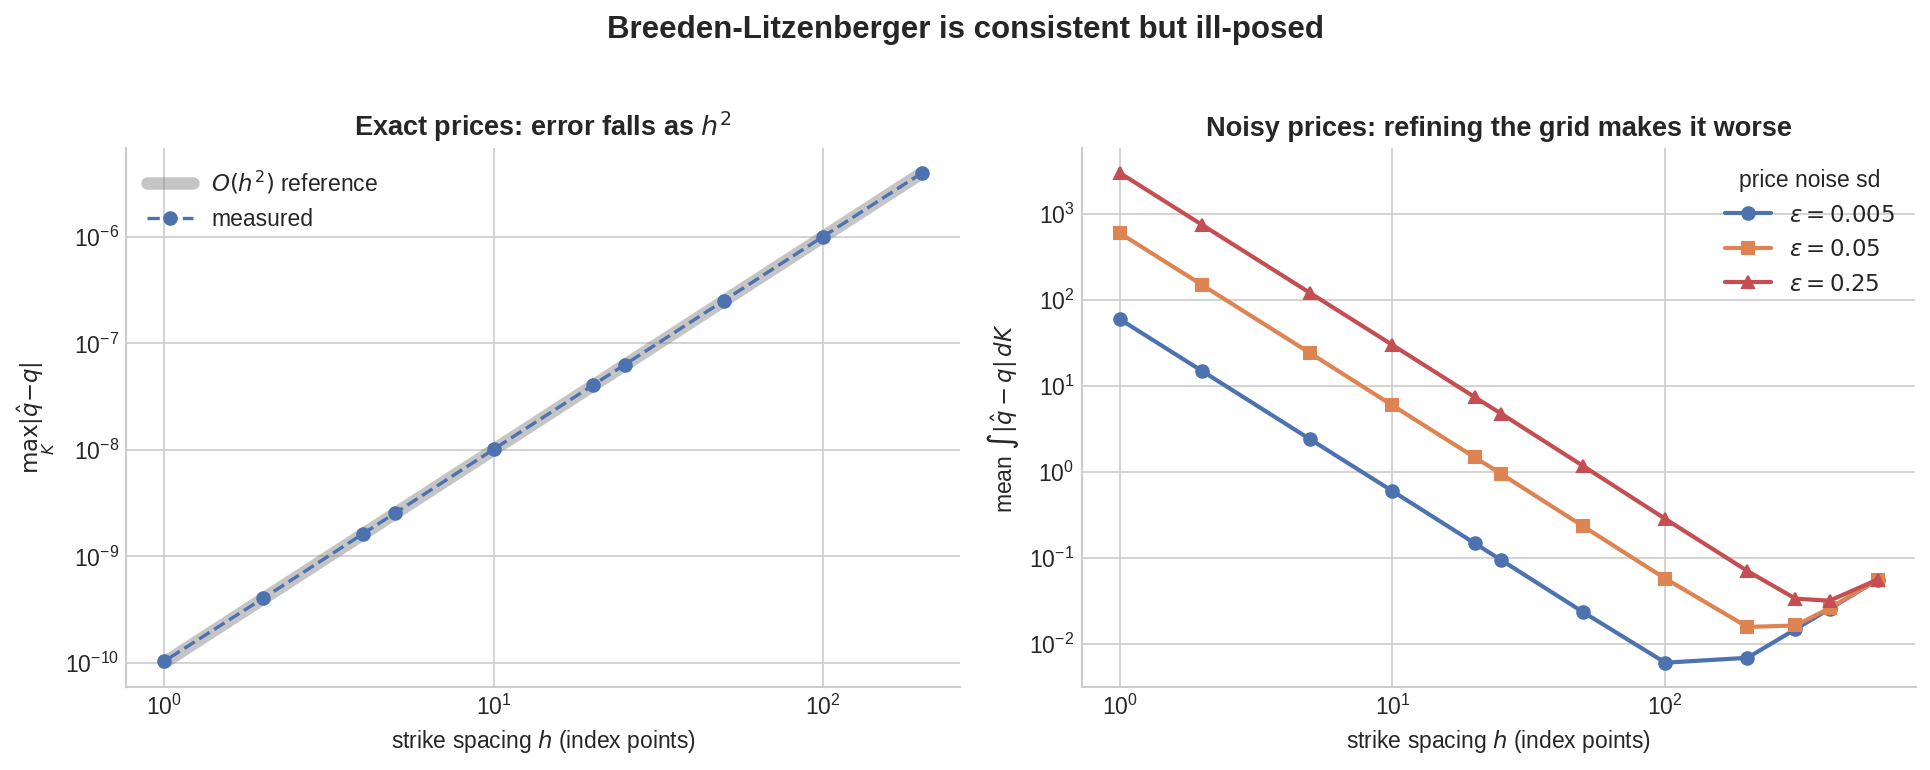
\includegraphics[width=\linewidth]{figures/01_convergence.png}
\caption{Left: on exact prices the error falls as $O(h^2)$, the grey reference
lying underneath the measured points. Right: with quote noise the error is
U-shaped in $h$, and refining the grid past $h^\star$ makes matters worse. The
two panels together are the argument for regularisation.}
\label{fig:convergence}
\end{figure}

\paragraph{Heston: a non-lognormal truth.} Black--Scholes is a forgiving test
because it has no smile. We therefore repeat the exercise under Heston
($v_0=0.04$, $\kappa=2$, $\theta=0.045$, $\sigma_v=0.55$, $\rho=-0.75$;
Feller deliberately violated, as real calibrations usually are). Prices come
from Gil-Pelaez inversion of the characteristic function in the
\citet{albrecher2007} formulation; the true density comes from inverting the
same characteristic function directly. Recovery on a 25-point grid gives $L^1$
error $2.0\times10^{-4}$ and $L^\infty$ error $2.6\times10^{-7}$, with the
negative skew correctly reproduced. As a further check, Heston collapses onto
Black--Scholes as $\sigma_v\to0$ to within $6.7\times10^{-7}$ in price.

\section{Data}
\label{sec:data}

A single CBOE delayed-quote snapshot of SPX and SPXW options, 29{,}858
contracts across 57 expiries, with quotes as of the close on 25 September 2026
and the index at $7743.41$. We use SPX monthlies, which are European and
AM-settled -- Breeden--Litzenberger assumes European exercise, so SPY, being
American, is unusable for this purpose. Daily S\&P 500 closes from 1927 and
daily VIX closes from 1990 supply the time-series half.

Rather than importing an external discount curve we recover the forward and
discount factor from the quotes themselves, regressing the parity spread
$C-P$ on $K$ over strikes within $5\%$ of spot, weighted by inverse quote width.
This is self-consistent: it returns the discount rate the option market is
actually using.

\begin{table}[htbp]
\centering
\small
\begin{tabular}{lrrrrrrr}
\toprule
Expiry & $T$ & strikes & $F$ & $D$ & implied $r$ & implied $q_d$ & parity RMSE \\
\midrule
2026-10-16 & 0.0575 & 482 & 7756.6 & 0.99754 & 4.29\% & 1.33\% & 0.078 \\
2026-11-20 & 0.1534 & 458 & 7782.6 & 0.99306 & 4.54\% & 1.25\% & 0.147 \\
2026-12-18 & 0.2301 & 455 & 7803.3 & 0.98965 & 4.52\% & 1.17\% & 0.108 \\
\bottomrule
\end{tabular}
\caption{Put-call parity diagnostics. Implied rates and dividend yields are
outputs, not inputs; the dividend yields near $1.2\%$ are correct for SPX.
Parity residuals of $0.1$ index points on a $7800$ index are about 1.3 basis
points.}
\label{tab:parity}
\end{table}

All subsequent cross-sectional work uses the December 2026 expiry, the longest
monthly and therefore the widest in strikes and the best behaved for kernel
estimation.

\section{The arbitrage-free surface and the risk-neutral density}
\label{sec:surface}

\subsection{The naive estimator fails as predicted}

Applying \eqref{eq:estimator} directly to December mid quotes on the
five-point strike grid, with a median half-spread of $0.65$:
Proposition~\ref{prop:noise} predicts a noise standard deviation of
$3.7\times10^{-2}$ in $\hat q$, against a peak density of $7.9\times10^{-4}$
implied by the $13.5\%$ ATM volatility. The noise-to-signal ratio is $47$, and
$39\%$ of the extracted density is negative (Figure~\ref{fig:naive}). Raw mids
also violate convexity at $35\%$ of adjacent strike triples.

\begin{figure}[htbp]
\centering
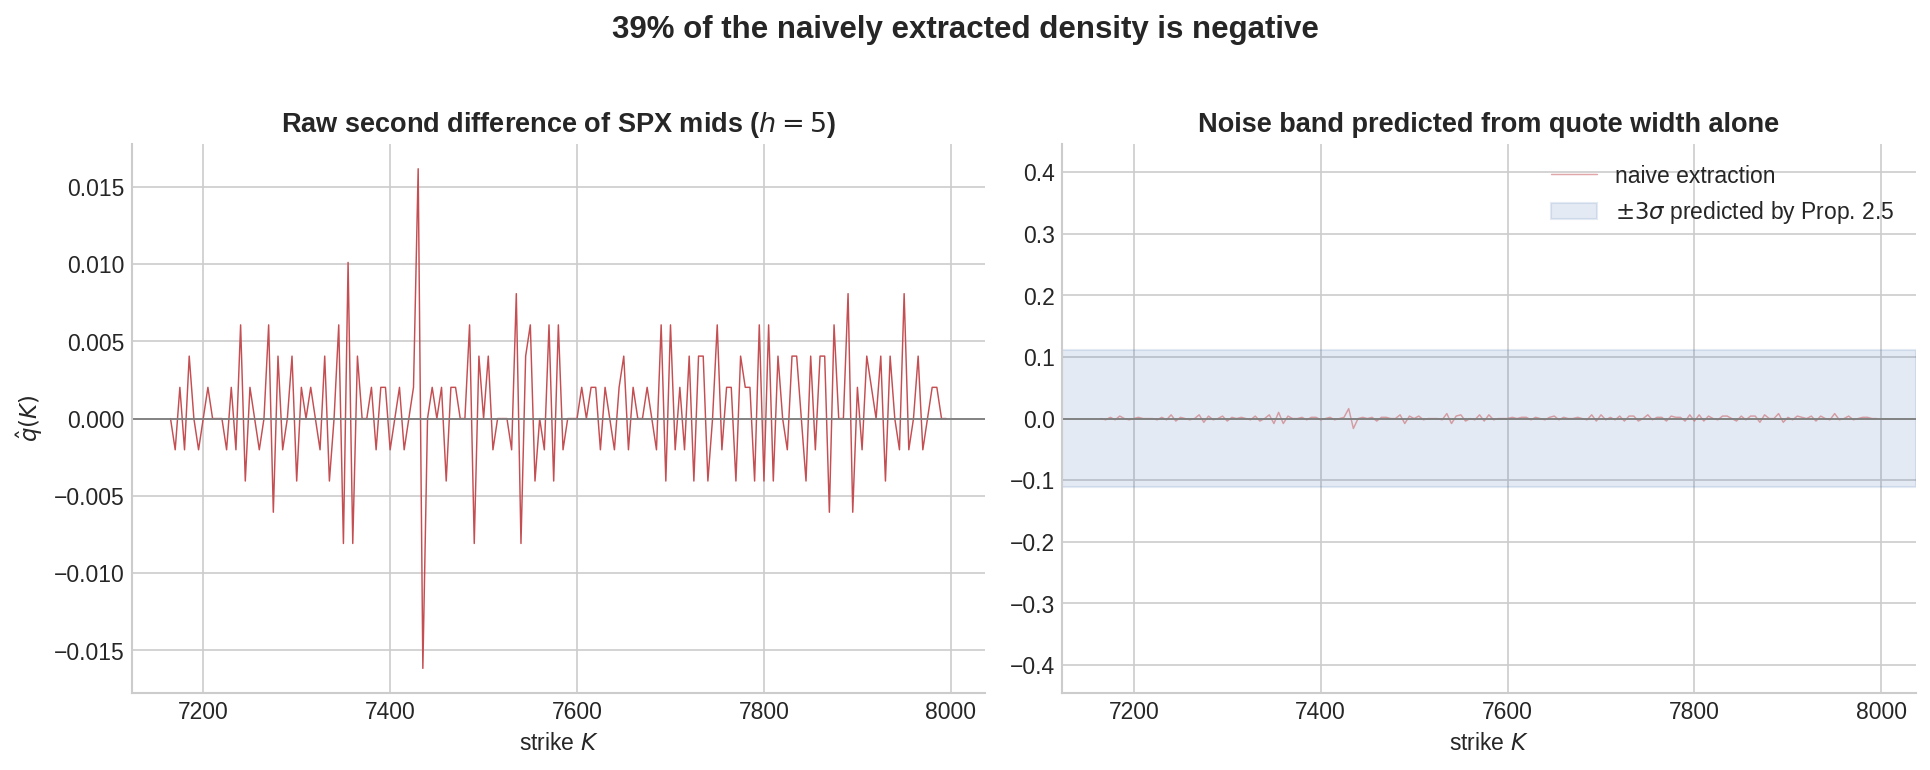
\includegraphics[width=\linewidth]{figures/06_naive_bl_failure.png}
\caption{Naive second differencing of SPX December mids. The shaded band is the
$\pm3\sigma$ region predicted by Proposition~\ref{prop:noise} from the quote
width alone, with no fitting. The estimator is not noisy; it is noise.}
\label{fig:naive}
\end{figure}

The measured $39\%$ negative fraction falls short of the $49\%$ predicted under
i.i.d.\ errors. Inverting the measured fraction implies an effective
independent noise of $0.028$ index points against $0.375$ implied by the
spread. Quote errors are therefore strongly positively correlated across
adjacent strikes -- consistent with market makers quoting from a common fitted
smile -- and the second difference cancels most of the common component. The
i.i.d.\ model is conservative here, not optimistic.

\subsection{Constrained SVI}

We fit raw SVI \citep{gatheral2004} in total variance,
$w(k) = a + b[\rho(k-m)+\sqrt{(k-m)^2+s^2}]$ with $k=\log(K/F)$, under hard
constraints: $b\ge0$, $s>0$, $w>0$, Lee's wing bound $b(1+|\rho|)\le2$
\citep{lee2004}, and the \citet{gatheral2014} butterfly condition $g(k)\ge0$ on
a dense grid extending $25\%$ beyond the data. We parameterise $\rho$ as
$\tanh(\cdot)$ so $|\rho|<1$ holds structurally, and use sixteen random starts
since the objective is not convex. Observations are weighted by inverse
variance, propagating the quote half-width into total-variance units via
$\dd w = 2\sigma T\,\dd C/\text{vega}$.

The density is then read off analytically,
\begin{equation}
q(K) = \frac{g(k)}{K\sqrt{2\pi w(k)}}\exp\!\left(-\tfrac12 d_2^2\right),
\qquad d_2 = -\frac{k}{\sqrt{w}}-\frac{\sqrt{w}}{2},
\end{equation}
verified against finite differences of the fitted slice's own call prices to
$1.7\times10^{-6}$ relative. No market data is differentiated at any point.

\paragraph{Quote reliability filter.} We drop 29 of 455 quotes priced below
\$1 or with relative spread above $15\%$. These extend to $k=-1.72$, roughly 26
standard deviations out at this maturity, trading near fifty cents with spreads
exceeding $30\%$ of price; their implied volatilities are a tick-size artefact.
This is a stated modelling choice, not data cleaning. The fitted range is
$k\in[-0.774,+0.132]$.

\begin{figure}[htbp]
\centering
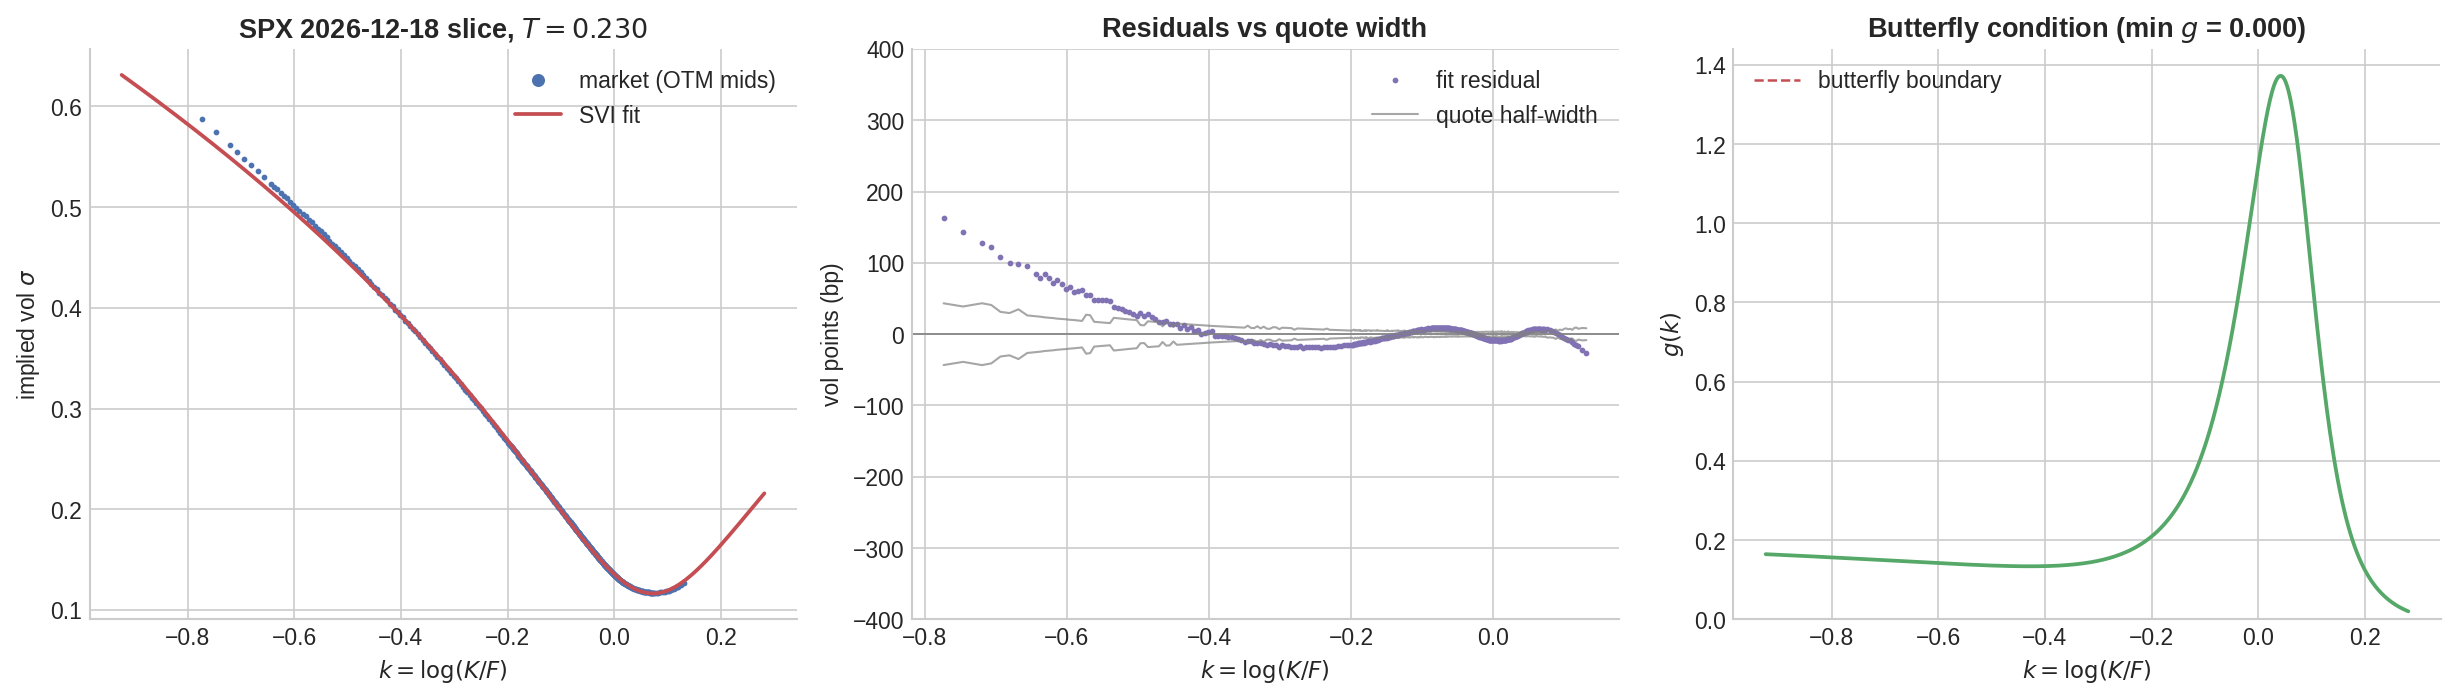
\includegraphics[width=\linewidth]{figures/07_svi_fit.png}
\caption{Fitted slice, residuals against the quote half-width, and the
butterfly function $g$. The fit sits inside the quote band from $k\approx-0.4$
upward; the error is concentrated in the deep left wing.}
\label{fig:svi}
\end{figure}

\begin{table}[htbp]
\centering
\small
\begin{tabular}{lrrr}
\toprule
Region & $n$ & RMSE (bp) & inside bid-ask \\
\midrule
core, $|k|\le0.15$ & 288 & 6.6 & 26.7\% \\
left, $-0.5\le k<-0.15$ & 104 & 13.5 & 22.1\% \\
deep left, $k<-0.5$ & 34 & 77.7 & 0.0\% \\
\midrule
all & 426 & 23.6 & 23.5\% \\
\bottomrule
\end{tabular}
\caption{Fit error by moneyness. The aggregate figure is misleading alone: in
the core the fit is 6.6 bp, and essentially all the error lives in the deep
left wing, where raw SVI's asymptotically \emph{linear} total variance cannot
match the observed \emph{concave} wing. The low inside-spread fractions reflect
a median SPX quote half-width of only 3.9 bp.}
\label{tab:svifit}
\end{table}

Fitted parameters are $a=-0.0227$, $b=0.1052$, $\rho=-0.0830$, $m=0.0520$,
$s=0.2459$. The resulting density has total mass $0.99997$ and a mean within
$0.56$ index points of the forward ($7\times10^{-5}$ relative), with skewness
$-1.99$ and excess kurtosis $16.0$. Neither the mass nor the mean is imposed by
the fit, so both are genuine checks: a five-parameter family is under no
obligation to integrate correctly.

\section{The physical density and the pricing kernel}
\label{sec:kernel}

\subsection{Two estimators of $p$}

The horizon is 59 NYSE sessions, $T = 0.2301$. We estimate $p$ two ways.

The \emph{naive} estimator is a Gaussian kernel density on overlapping 59-day
log returns since 1990. It is unconditional. Its nominal $n=9{,}192$ is
$156$ independent observations in disguise, since 59-day returns sampled daily
overlap by 58 of 59 days.

The \emph{filtered} estimator follows \citet{baroneadesi2008}: fit GARCH(1,1)
with Student-$t$ innovations to daily returns, then bootstrap standardised
residuals forward 59 days from \emph{today's} conditional variance. The fit
gives $\alpha=0.102$, $\beta=0.892$, persistence $0.994$, $\nu=6.15$, with an
unconditional volatility of $23.4\%$ against a current conditional volatility of
$11.6\%$; the simulated horizon distribution mean-reverts upward and lands at
$13.8\%$ annualised, with skewness $-0.81$ and kurtosis $9.4$.

\begin{remark}[Centring the residual pool]
Standardised residuals do not have mean zero in sample, because high-variance
days carry systematically signed residuals. Bootstrapping them raw injects an
uncontrolled drift on top of the mean parameter. Centring the pool makes the
horizon drift exactly $\mu h$, so the drift becomes an explicit assumption
rather than an artefact of the filter. This was detected because the base case
and a nominally identical sensitivity scenario disagreed.
\end{remark}

\begin{figure}[htbp]
\centering
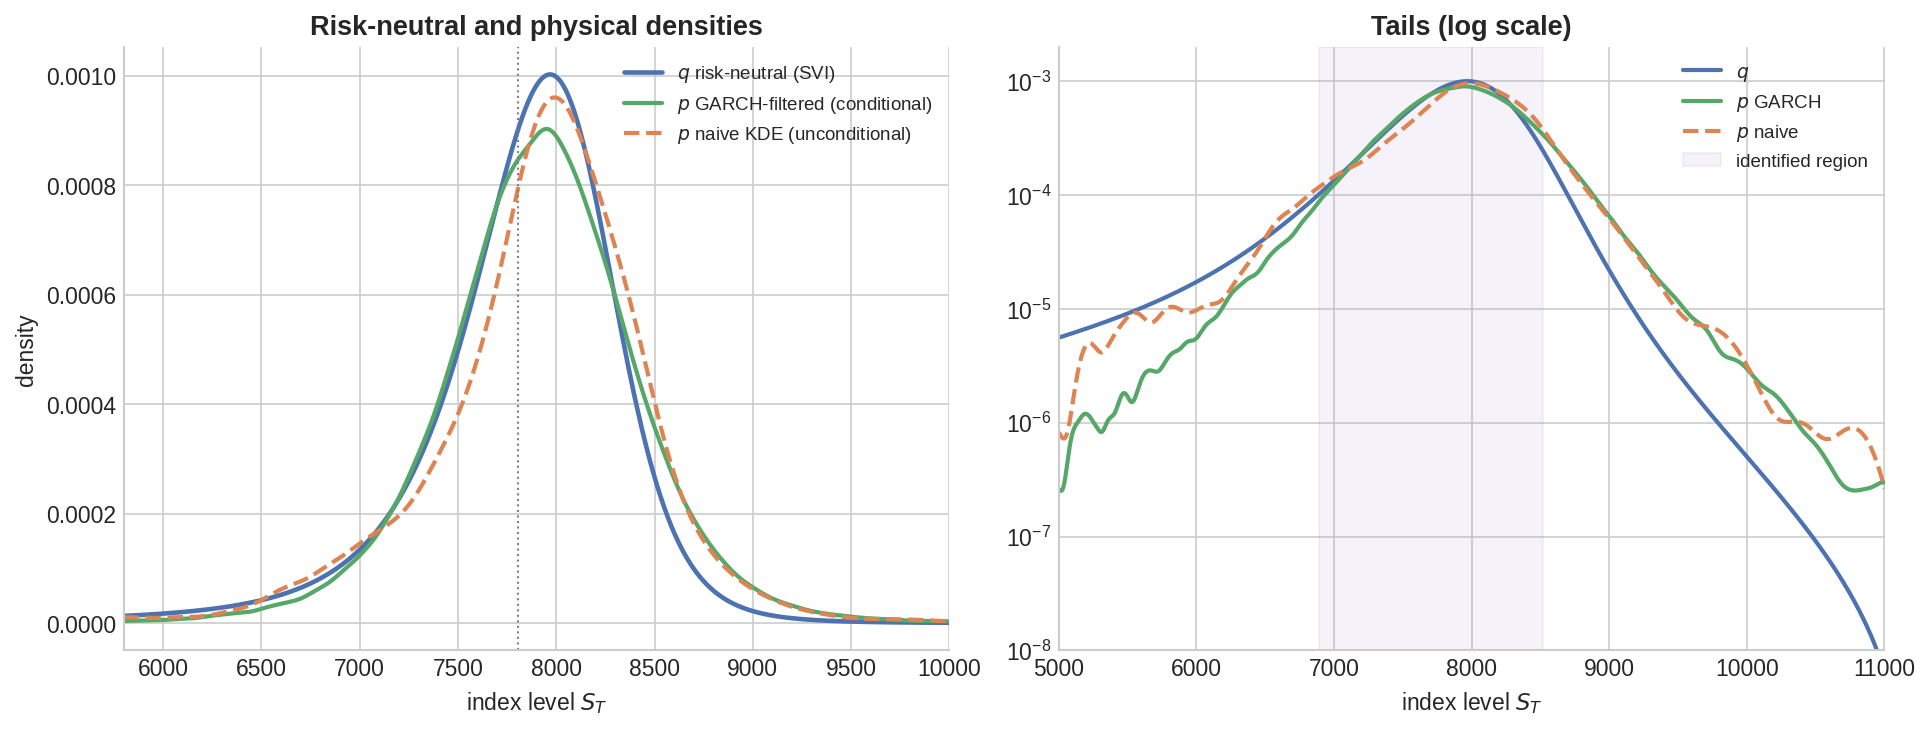
\includegraphics[width=\linewidth]{figures/09_densities.png}
\caption{Risk-neutral and physical densities. $q$ has the fatter left tail and
the thinner right tail: the market prices drawdowns above their historical
frequency and rallies below it.}
\label{fig:densities}
\end{figure}

The premium is visible directly in tail probabilities: $\Q(S_T<7000) = 6.20\%$
against $\PP = 3.96\%$ (ratio $1.56$), while $\Q(S_T>8700) = 2.02\%$ against
$\PP = 5.41\%$ (ratio $0.37$). That asymmetry is the kernel.

\subsection{The kernel, and why its shape is not identified}

On the identified region -- the central $90\%$ of $q$, $[6893,8518]$ -- the
estimated kernel \eqref{eq:kernel} is non-monotone: increasing over $41.3\%$ of
the region with the filtered $p$ and $39.8\%$ with the naive one. Taken at face
value this is the pricing kernel puzzle.

It should not be taken at face value. The physical drift enters $p$ directly
and is the least well determined input in the exercise: the 1990--2026 sample
mean is $8.41\%$ per year with a standard error of $2.97\%$, a $95\%$ interval
of $[2.59\%, 14.23\%]$.

\begin{table}[htbp]
\centering
\small
\begin{tabular}{lrr}
\toprule
Drift scenario & $\mu$ (annual) & fraction of region increasing \\
\midrule
$\hat\mu - 2\,$s.e. & 2.47\% & 51.8\% \\
risk-neutral drift & 3.35\% & 50.2\% \\
$\hat\mu$ & 8.41\% & 39.9\% \\
$\hat\mu + 2\,$s.e. & 14.35\% & \textbf{2.7\%} \\
GARCH constant mean & 18.93\% & 2.2\% \\
\bottomrule
\end{tabular}
\caption{Sensitivity of kernel monotonicity to the assumed physical drift.
Within the $95\%$ interval of the equity premium the verdict reverses
completely.}
\label{tab:drift}
\end{table}

\begin{figure}[htbp]
\centering
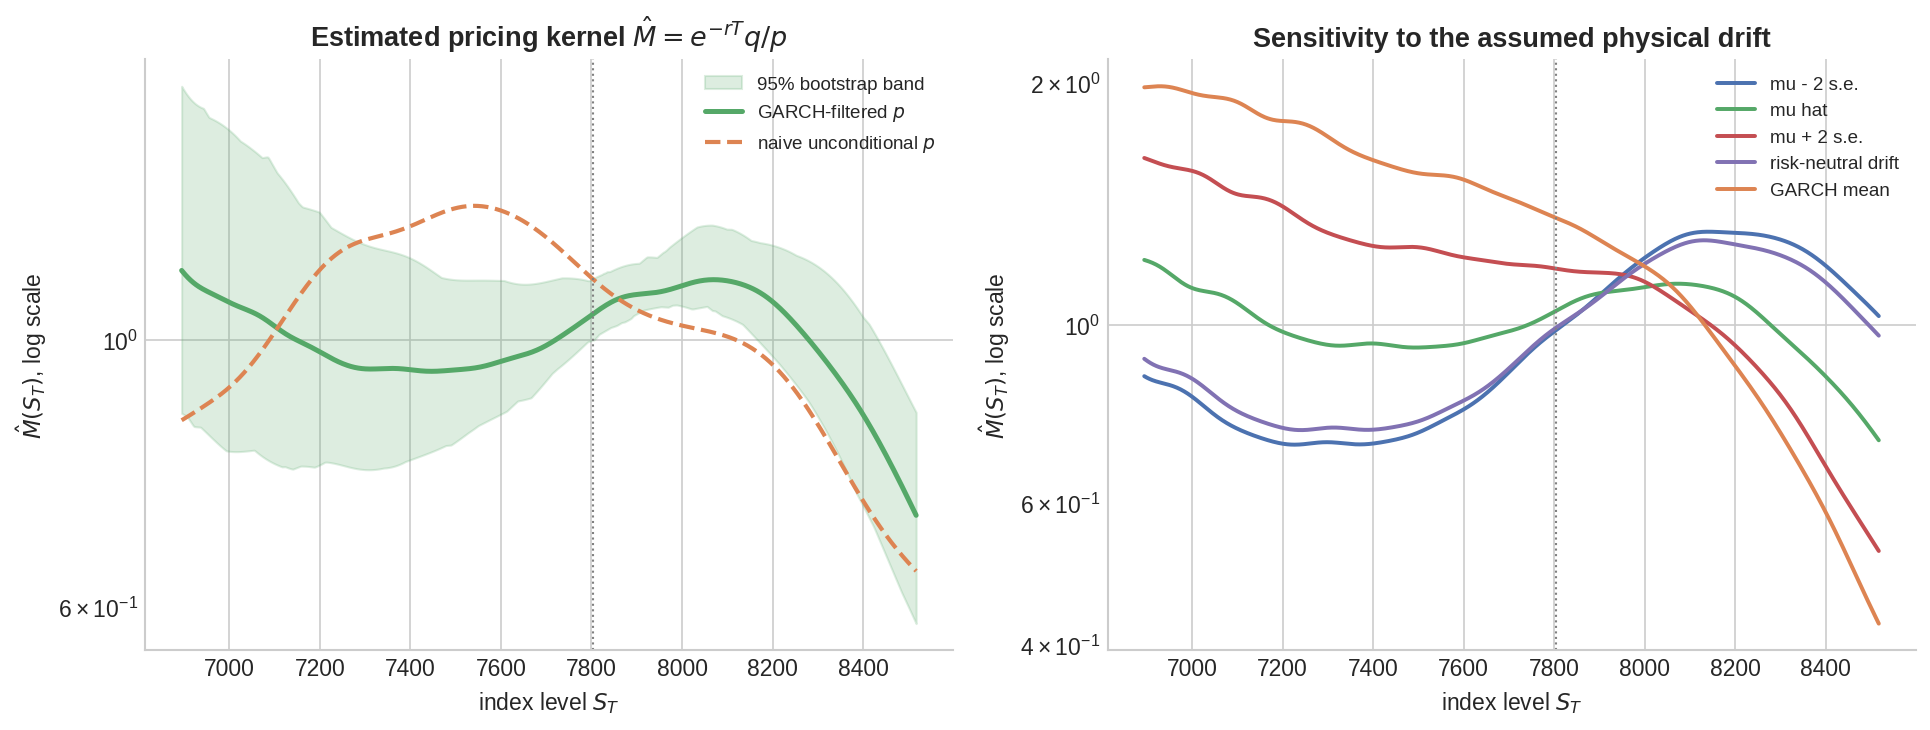
\includegraphics[width=\linewidth]{figures/10_pricing_kernel.png}
\caption{Left: estimated kernel with a $95\%$ bootstrap band over 120 resamples
of the residual pool. Right: the same kernel under drift assumptions spanning
the equity premium's confidence interval. The shape is set by the drift, not by
the option data.}
\label{fig:kernel}
\end{figure}

At the top of the interval the kernel is essentially monotone decreasing,
exactly as theory predicts; at the bottom it is strongly non-monotone. We
therefore cannot reject monotonicity. The bootstrap band in
Figure~\ref{fig:kernel} reaches the same conclusion by a different route: it is
wide enough to contain a monotone decreasing kernel across most of the region.

One trap deserves comment. The GARCH constant-mean estimate is $18.93\%$ per
year against an $8.41\%$ sample mean, because GARCH weights low-variance days
most heavily and low-variance days are bull markets. It is biased upward as an
equity premium estimate. It also sits ready-made in the fitted object, and
using it -- as a naive pipeline would -- produces a cleanly monotone kernel for
entirely the wrong reason.

\section{Model-free implied variance and the variance risk premium}
\label{sec:vrp}

\subsection{Reconstructing the VIX}

The snapshot's SPXW expiries at 28 and 35 days bracket 30, so \eqref{eq:vix}
can be run on our own chain and checked against the published index. Following
the CBOE recipe exactly -- forward from the strike with the smallest $|C-P|$,
$K_0$ the largest strike below it, OTM options subject to the
two-consecutive-zero-bid stopping rule, and interpolation in total variance --
we obtain
\[
\text{VIX}_{\text{reconstructed}} = 14.880
\qquad\text{against}\qquad
\text{VIX}_{\text{published}} = 14.87,
\]
an error of $+0.07\%$. This validates the derivation and the implementation
together, and licenses using the published VIX history as a model-free implied
variance series -- which is what makes a 36-year time series possible from a
single option snapshot.

\paragraph{Truncation, quantified.} The $1/K^2$ weight loads on deep OTM puts,
exactly where chains run out. The share of the variance sum by moneyness is
$4.6\%$ for $K/F<0.70$, $9.1\%$ for $0.70$--$0.85$, $19.8\%$ for
$0.85$--$0.95$, $64.3\%$ for $0.95$--$1.05$ and $2.1\%$ above. So $4.6\%$ of
the answer comes from the region most exposed to truncation.

\subsection{The jump correction}

Refitting the 35-day slice through the Section~\ref{sec:surface} pipeline, the
risk-neutral log return has variance $0.00242$ and third central moment
$-4.46\times10^{-4}$ (skewness $-3.74$). Applying \eqref{eq:jump}:

\begin{center}
\small
\begin{tabular}{lr}
\toprule
log-contract implied volatility & 15.90\% \\
jump-corrected $\sqrt{\E[\text{QV}]}$ & 14.89\% \\
correction as share of implied variance & 12.3\% \\
\bottomrule
\end{tabular}
\end{center}

Scaled to the sample mean implied variance, the correction is $0.00537$ in
variance units against a measured mean premium of $0.01136$ -- roughly $47\%$
of the measured premium is the jump term rather than compensation for variance
risk. Two caveats travel with that figure: it is extrapolated from a single
cross-section, and it is an \emph{upper bound}, since attributing the entire
third moment to jumps ignores that a leverage-driven stochastic-volatility
diffusion generates negative skew without any jumps at all.

\subsection{Testing the premium}

We form $\VRP_t = \IV_t^2 - \RV_t^2$ with $\IV$ the VIX and $\RV$ the
subsequently realised variance over 21 sessions, giving 9{,}226 daily
observations from 1990 to 2026. Mean implied volatility is $20.9\%$ against
mean subsequently realised volatility of $18.0\%$.

\begin{table}[htbp]
\centering
\small
\begin{tabular}{lrrrr}
\toprule
Specification & lags & mean & s.e. & $t$ \\
\midrule
Naive, no HAC & 0 & 0.01136 & 0.00053 & \textbf{21.30} \\
Newey--West, lag = window & 21 & 0.01136 & 0.00206 & 5.52 \\
Newey--West, lag = $2\times$ window & 42 & 0.01136 & 0.00232 & 4.90 \\
Newey--West, Andrews plug-in & 196 & 0.01136 & 0.00228 & 4.99 \\
\bottomrule
\end{tabular}
\caption{Mean variance risk premium and standard errors. Overlapping windows
make the series autocorrelated by construction even under the null; HAC
inflates the standard error $3.9\times$ and the $t$-statistic falls from 21.3 to
about 5. Lag selection follows \citet{newey1987,newey1994}.}
\label{tab:hac}
\end{table}

The premium survives, but a paper reporting $21.3$ would be reporting an
artefact of overlap.

\begin{figure}[htbp]
\centering
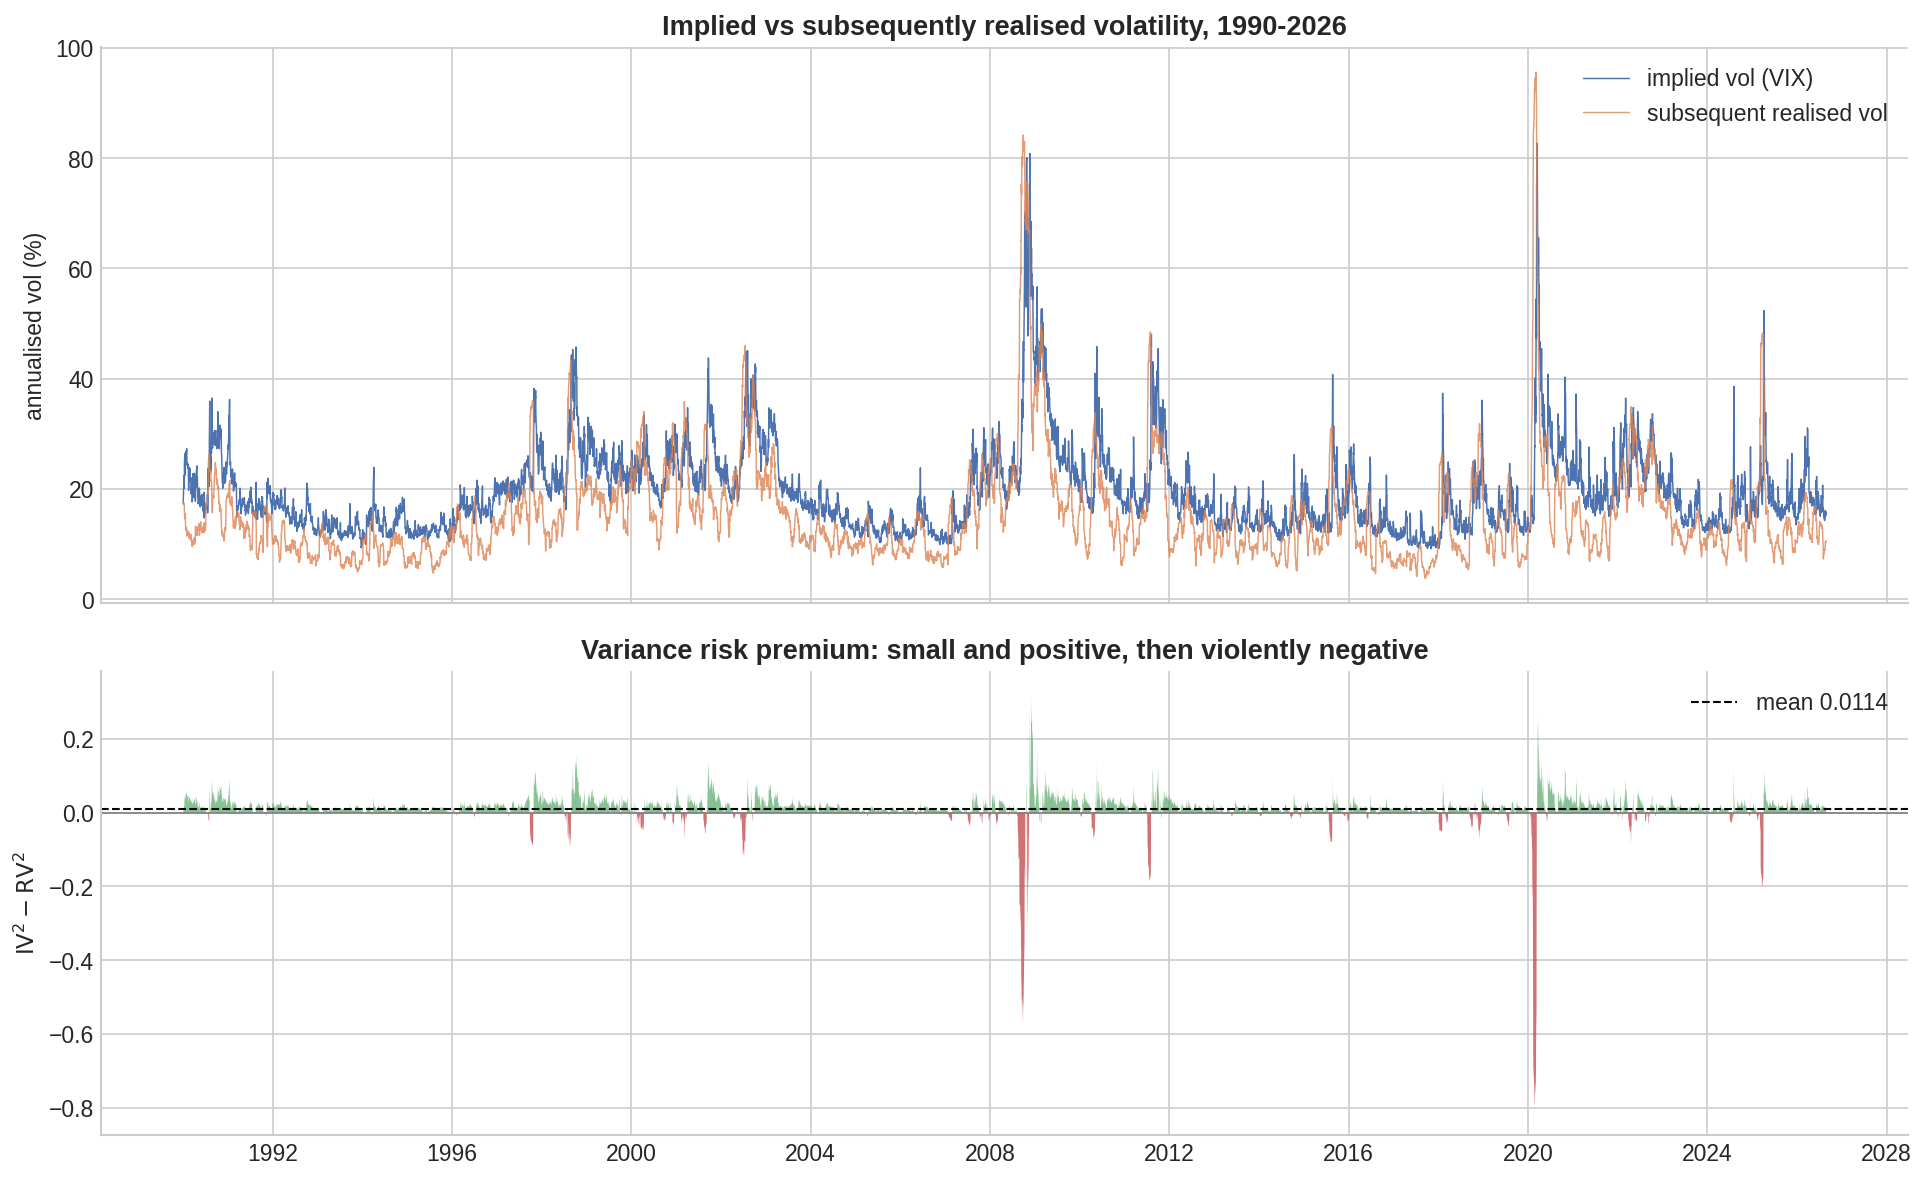
\includegraphics[width=\linewidth]{figures/11_vrp_timeseries.png}
\caption{Implied versus subsequently realised volatility, and the resulting
premium. Positive most of the time; violently negative in 2008 and 2020.}
\label{fig:vrp}
\end{figure}

\subsection{Shape, and why the mean is a weak summary}

The premium is positive on $85.9\%$ of days, with skewness $-8.38$ and excess
kurtosis $109$. The worst observation, $-0.816$, is 26 February 2020. The worst
$1\%$ of days subtract $33\%$ of the total earned by the other $99\%$. This is
the short-volatility payoff profile quantified: steady accumulation punctuated
by losses large enough to dominate the average.

\begin{figure}[htbp]
\centering
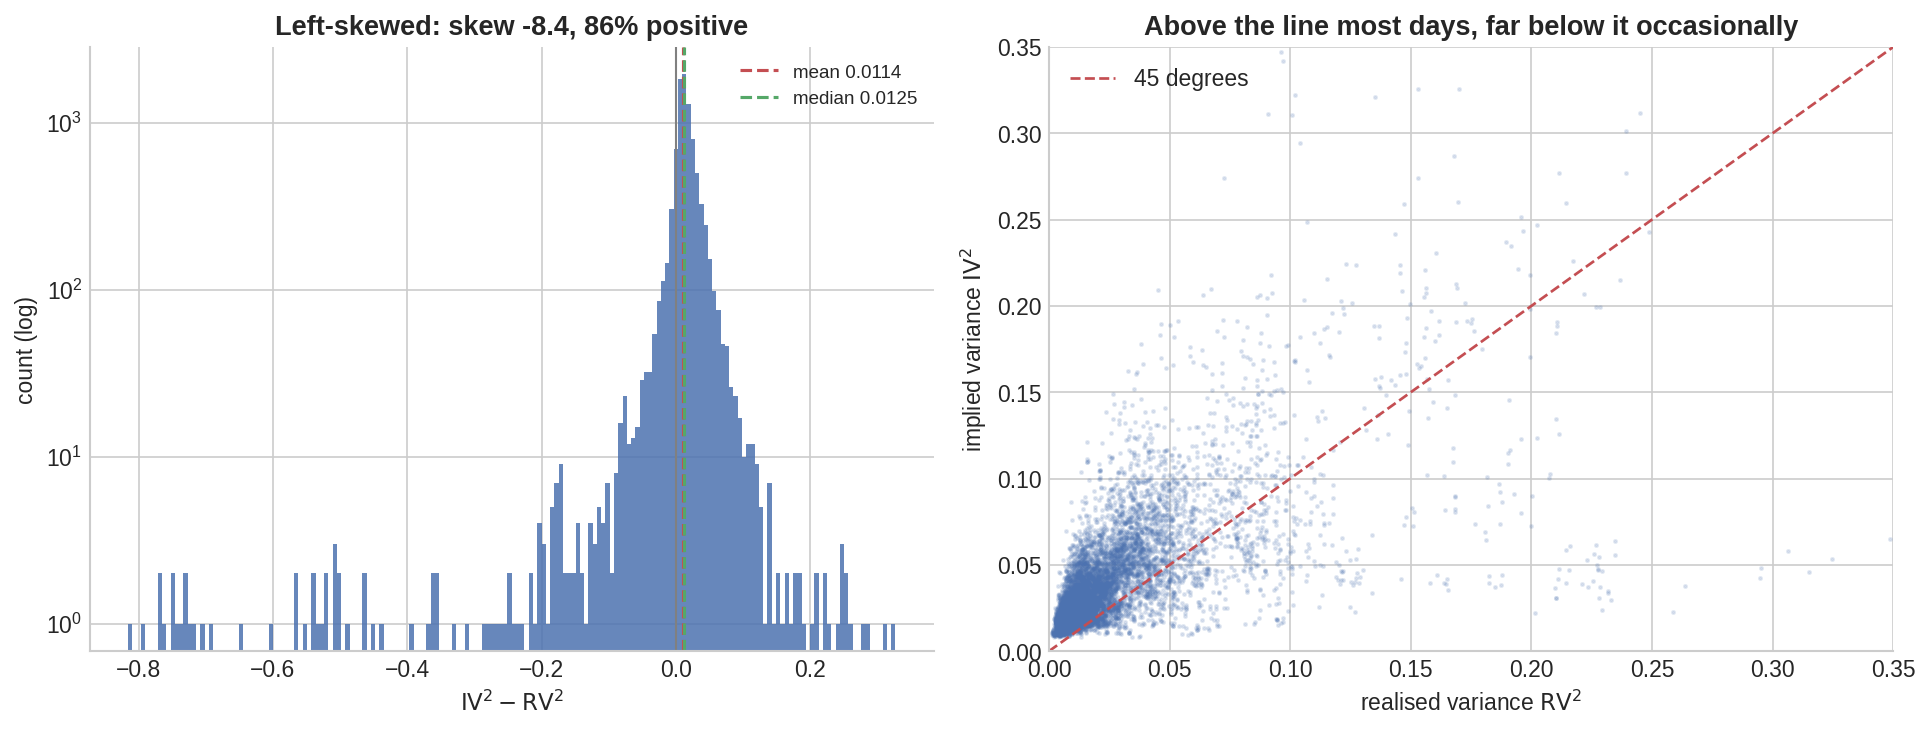
\includegraphics[width=\linewidth]{figures/12_vrp_distribution.png}
\caption{Distribution of the premium (log count scale) and the implied-realised
scatter. Above the 45-degree line most days, far below it occasionally.}
\label{fig:vrpdist}
\end{figure}

By decade the premium is not uniformly significant: $t_{NW} = 11.18$
(1990--99), $1.97$ (2000--09), $5.72$ (2010--19), $0.93$ (2020--26), with the
point estimate more than halving since the 1990s. Two of four subperiods fail at
the $5\%$ level. Pooling into a single comfortable number would conceal this.

\section{Limitations}
\label{sec:limits}

\paragraph{Wing extrapolation and truncation.} SVI extrapolates beyond the last
quoted strike by construction. For the December density only
$1.5\times10^{-4}$ of total mass lies outside the quoted range, so the reported
moments barely depend on extrapolation; but the density should be read only on
the quoted range. One artefact: beyond $K\approx11{,}200$, well past the last
quote at $10{,}600$, the fitted density dips to near zero and recovers because
the butterfly constraint binds at the edge of the padded grid. The mass involved
is $O(10^{-7})$ and affects no reported figure, but it is named rather than
cropped. For the variance swap the truncation exposure is larger: $4.6\%$ of the
sum comes from $K/F<0.70$.

\paragraph{Overlapping returns.} Both the physical density and the variance risk
premium use overlapping windows. For $p$, the nominal 9{,}192 observations are
$156$ effective ones; we therefore prefer the filtered estimator, which does not
rely on overlapping samples at all. For the premium, HAC inference inflates the
standard error $3.9\times$. Silverman's bandwidth rule, used for the naive KDE,
assumes independence and undersmooths badly here; we report the estimator
without an ad hoc correction rather than choose an arbitrary one.

\paragraph{Functional-form error in the wing.} Raw SVI has asymptotically linear
total variance; the observed SPX left wing is concave. Fit error reaches $77.7$
bp for $k<-0.5$ against $6.6$ bp in the core. A more flexible parameterisation,
or a constrained spline, would reduce this; five parameters cannot.

\paragraph{One cross-section, one maturity.} All cross-sectional results use a
single snapshot and, for the kernel, a single expiry. There is no term structure
of the kernel here and no time-series variation in $q$. The jump correction's
extrapolation to the sample mean is correspondingly heroic.

\paragraph{The projection is not the kernel.} By
Proposition~\ref{prop:projection} we recover $\E^\PP[\xi\mid S_T]$, not $\xi$.
Any component orthogonal to the terminal index level is invisible, so
non-monotonicity may reflect an omitted state variable rather than a violation
of theory.

\paragraph{Identification of the drift.} The dominant limitation. As
Table~\ref{tab:drift} shows, the qualitative conclusion about monotonicity is
determined by an input estimated with a $2.97\%$ annual standard error. No
amount of care on the option side repairs this.

\section{Conclusion}
\label{sec:conclusion}

We estimated the projected Radon--Nikodym derivative from SPX options,
validating every step against a known answer first. The Breeden--Litzenberger
estimator is consistent at order $h^2$ with a leading constant we verify to
$4\times10^{-5}$, and ill-posed with a noise amplification we derive and then
confirm on live quotes, where the naive extraction is $47$ times more noise than
signal. Arbitrage-constrained SVI removes the problem, yielding a density that
integrates to $0.99997$ and reprices the forward to $7\times10^{-5}$.

The estimated pricing kernel is non-monotone at the point estimate. We do not
claim to have found the pricing-kernel puzzle, because the same data with a
drift two standard errors higher produces a monotone decreasing kernel. The
honest statement is that the shape is not identified at this sample size.

On the variance side, reconstructing the VIX to $0.07\%$ from our own chain
validates the log-contract derivation end to end. The premium is positive and
significant under HAC inference, but $47\%$ of its measured magnitude is
plausibly a jump correction rather than variance risk compensation, its
$t$-statistic falls from $21.3$ to $5.5$ once overlap is handled, and two of
four decades fail at conventional levels.

\paragraph{Reproducibility.} All figures and tables are produced by five
numbered scripts run in sequence; no result in this paper is hand-copied.

\begin{thebibliography}{99}
\small

\bibitem[Aït-Sahalia and Lo(2000)]{aitsahalia2000}
Aït-Sahalia, Y. and A. Lo (2000). Nonparametric risk management and implied
risk aversion. \emph{Journal of Econometrics} 94, 9--51.

\bibitem[Albrecher et al.(2007)]{albrecher2007}
Albrecher, H., P. Mayer, W. Schoutens and J. Tistaert (2007). The little Heston
trap. \emph{Wilmott Magazine}, January, 83--92.

\bibitem[Bakshi et al.(2003)]{bakshi2003}
Bakshi, G., N. Kapadia and D. Madan (2003). Stock return characteristics, skew
laws, and the differential pricing of individual equity options.
\emph{Review of Financial Studies} 16, 101--143.

\bibitem[Barone-Adesi et al.(2008)]{baroneadesi2008}
Barone-Adesi, G., R. Engle and L. Mancini (2008). A GARCH option pricing model
with filtered historical simulation. \emph{Review of Financial Studies} 21,
1223--1258.

\bibitem[Bollerslev et al.(2009)]{bollerslev2009}
Bollerslev, T., G. Tauchen and H. Zhou (2009). Expected stock returns and
variance risk premia. \emph{Review of Financial Studies} 22, 4463--4492.

\bibitem[Breeden and Litzenberger(1978)]{breeden1978}
Breeden, D. and R. Litzenberger (1978). Prices of state-contingent claims
implicit in option prices. \emph{Journal of Business} 51, 621--651.

\bibitem[Carr and Madan(2001)]{carr2001}
Carr, P. and D. Madan (2001). Optimal positioning in derivative securities.
\emph{Quantitative Finance} 1, 19--37.

\bibitem[Carr and Wu(2009)]{carr2009}
Carr, P. and L. Wu (2009). Variance risk premiums. \emph{Review of Financial
Studies} 22, 1311--1341.

\bibitem[CBOE(2019)]{cboe2019}
Chicago Board Options Exchange (2019). \emph{Cboe Volatility Index (VIX) White
Paper}.

\bibitem[Gatheral(2004)]{gatheral2004}
Gatheral, J. (2004). A parsimonious arbitrage-free implied volatility
parameterization. Presentation, Global Derivatives \& Risk Management, Madrid.

\bibitem[Gatheral and Jacquier(2014)]{gatheral2014}
Gatheral, J. and A. Jacquier (2014). Arbitrage-free SVI volatility surfaces.
\emph{Quantitative Finance} 14, 59--71.

\bibitem[Heston(1993)]{heston1993}
Heston, S. (1993). A closed-form solution for options with stochastic
volatility. \emph{Review of Financial Studies} 6, 327--343.

\bibitem[Jackwerth(2000)]{jackwerth2000}
Jackwerth, J. (2000). Recovering risk aversion from option prices and realized
returns. \emph{Review of Financial Studies} 13, 433--451.

\bibitem[Lee(2004)]{lee2004}
Lee, R. (2004). The moment formula for implied volatility at extreme strikes.
\emph{Mathematical Finance} 14, 469--480.

\bibitem[Natenberg(1994)]{natenberg1994}
Natenberg, S. (1994). \emph{Option Volatility and Pricing}, 2nd ed. McGraw-Hill.

\bibitem[Newey and West(1987)]{newey1987}
Newey, W. and K. West (1987). A simple, positive semi-definite,
heteroskedasticity and autocorrelation consistent covariance matrix.
\emph{Econometrica} 55, 703--708.

\bibitem[Newey and West(1994)]{newey1994}
Newey, W. and K. West (1994). Automatic lag selection in covariance matrix
estimation. \emph{Review of Economic Studies} 61, 631--653.

\bibitem[Rosenberg and Engle(2002)]{rosenberg2002}
Rosenberg, J. and R. Engle (2002). Empirical pricing kernels. \emph{Journal of
Financial Economics} 64, 341--372.

\end{thebibliography}

\end{document}
